\documentclass[journal]{IEEEtran}

% *** CITATION PACKAGES ***
\usepackage[backend=biber,style=ieee]{biblatex} %bibliography with IEEE style.
\addbibresource{ref.bib} %Imports bibliography file
\bibliography{}

% *** GRAPHICS RELATED PACKAGES ***
\ifCLASSINFOpdf
  \usepackage[pdftex]{graphicx}
\else
\fi

% *** MATH PACKAGES ***
\usepackage{amsmath}
\usepackage{amssymb}
\usepackage{gensymb}
\usepackage{hyperref}

\begin{document}
%
% paper title
\title{ELEC6212: Wireless Sunflower Network}
\author{\IEEEauthorblockN{Benjamin~Dix-Matthews\IEEEauthorrefmark{1},
Georgios Psimenos\IEEEauthorrefmark{1},
Ganiyu AJ Ibraheem\IEEEauthorrefmark{1} and 
Aswin K Ramasubramanian\IEEEauthorrefmark{1}}
\IEEEauthorblockA{\IEEEauthorrefmark{1}University~of~Southampton}}

% The paper headers
\markboth{ELEC6212: Biologically Inspired Robotics}%
{University of Southampton}

% make the title area
\maketitle

% As a general rule, do not put math, special symbols or citations
% in the abstract or keywords.
\begin{abstract}
The idea of this project was to create a device capable of ultra-low power sensing and ultra-low power transmission that is capable of harvesting the energy required for its operation from solar sources. The energy harvesting nature of the device would eliminate the significant operational expenditure required to replace batteries in periphery nodes after they have gone flat. As batteries are typically known for having relatively short operational lifetimes (<10 years), our design would instead use a super capacitor in order to store the energy required for operation. This type of “Zero-Energy Sensing” is a new idea with huge potential in the IoT field.
\end{abstract}

\section{Introduction}
% The very first letter is a 2 line initial drop letter followed
% by the rest of the first word in caps.
\IEEEPARstart{T}{his} product would be aimed toward outdoor sensing applications where typical wireless sensing networks could be useful. A specific example of its usage would be a soil moisture detector for monitoring crops. The idea of the Wireless Sunflower Network would be to design a cheap product that could be easily set up by someone unfamiliar with electronics in order to build the sensing network (a plug and play solution).

\hfill bdm

\hfill April 25, 2018

\subsection{Definitions}
Internet of Things: IOT
% needed in second column of first page if using \IEEEpubid
%\IEEEpubidadjcol
\section{Motivation}

\section{Architecture}

\section{Communication}
LoRa is a low power, long range telecommunication technology that is ideal for the type of energy stringent wireless networks being considered. The physical layer of LoRa (Long Range) is a proprietary spread spectrum technique derived from Chirp Spread Spectrum (CSS) and is owned by Semtech~\cite{borLORAforIOT}. The standard MAC layer protocol is LoRaWAN and is an open standard being developed by the LoRa Alliance~\cite{ouluPetajajarvi}. As this protocol is open source, ad hoc networks can be set up without having to wait for a network provider. The transmission distance, energy usage and data rate are all dependent on five configurable parameters. The Semtech data sheets~\cite{lora:sx1272/73} specify how these parameters affect power usage.  Semtech also offer a calculator~\cite{loraCALCULATOR} that may be used to test individual parameter sets.



\section{Energy Harvesting}
\input{hardware.tex}

\section{Data Handling}
The data handling is organised into 3 sections: The first being a MongoDB data-store for handling all the incoming data from the flowers, the second being the dashboard for visualising the data available in the data-store and the last being a central server that communicates with a lora-module via serial-port, parsing and saving the lora packets and also acting as a web-server to the dashboard.

\subsection{MongoDB Data store}
% Quick intro to MongoDB (No-SQL)
MongoDB is a No-SQL database that provides an expressive query language and flexible data-store that allows iteration of data models. It is a highly efficient database that supports millions of operations per sec and can handle petabytes of data as well being able to scale (grow) horizontally with support for database clusters.

% Benefits of MongoDB (Rapid prototyping)
This rich feature set provided us with a strong foundation as a data-store for the sunflowers for two main reasons. Firstly, during the development stage, it provided us with a medium for rapid prototyping as we were able to rapidly change the schema of the data that was being stored and 
% Scalability and distributed nature which can support distributed sunflowers
due the distributed and highly scalable nature of MongoDB; It is theoretically possible for us to scale this data-store to support thousands of sunflowers.

\subsection{Dashboard}
% Brief intro to the dashboard as a valuable tool for analytics
The dashboard acts as an operator user-interface for navigating the data in the MongoDB data-store. One of the functionalities we encoded into it is support for analytics on the Sun flower data, this is illustrated in figure \ref{figure:home} where we aggregated data on the temperature and humidity.
\begin{figure}
	\centering
	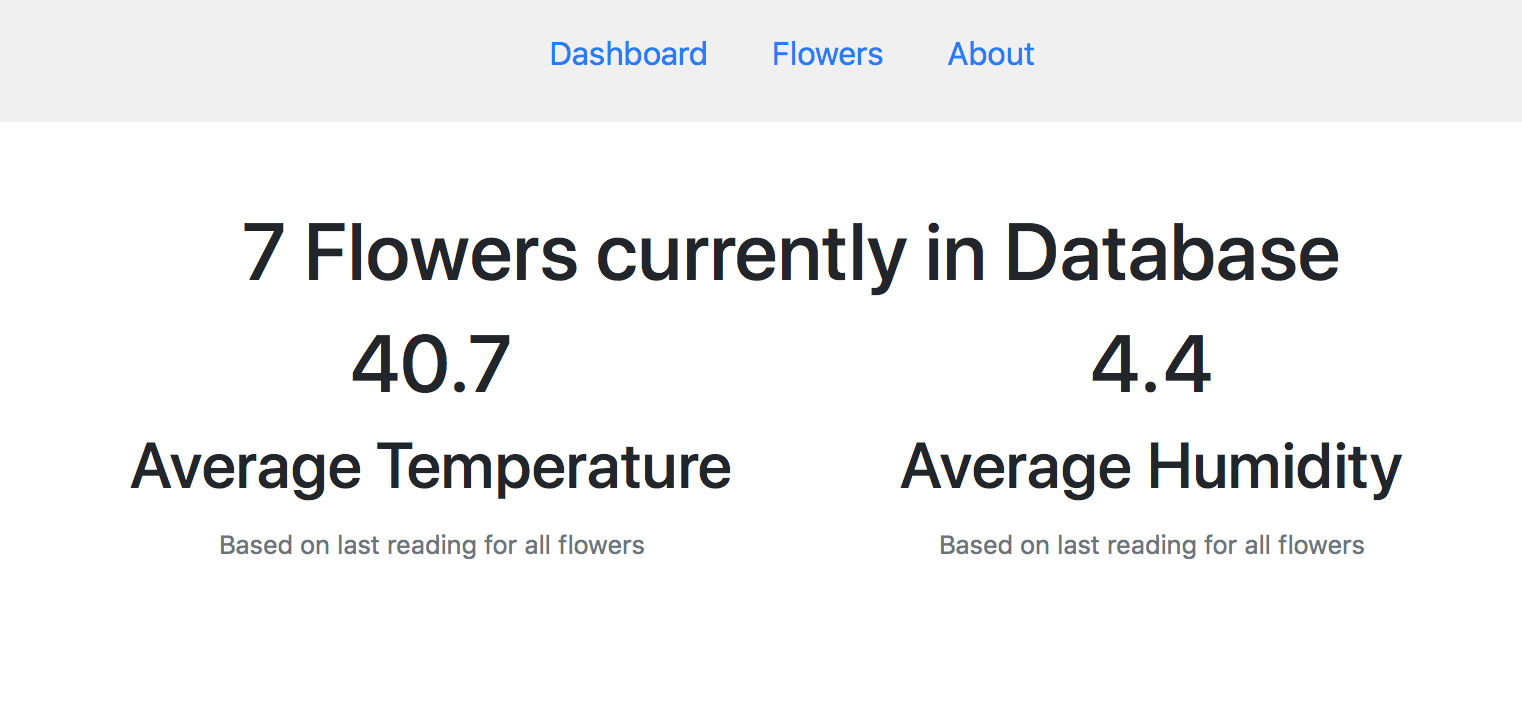
\includegraphics[width=\linewidth]{home}
	\caption{Homepage for the dashboard}
	\label{figure:home}
\end{figure}
\begin{figure}
	\centering
	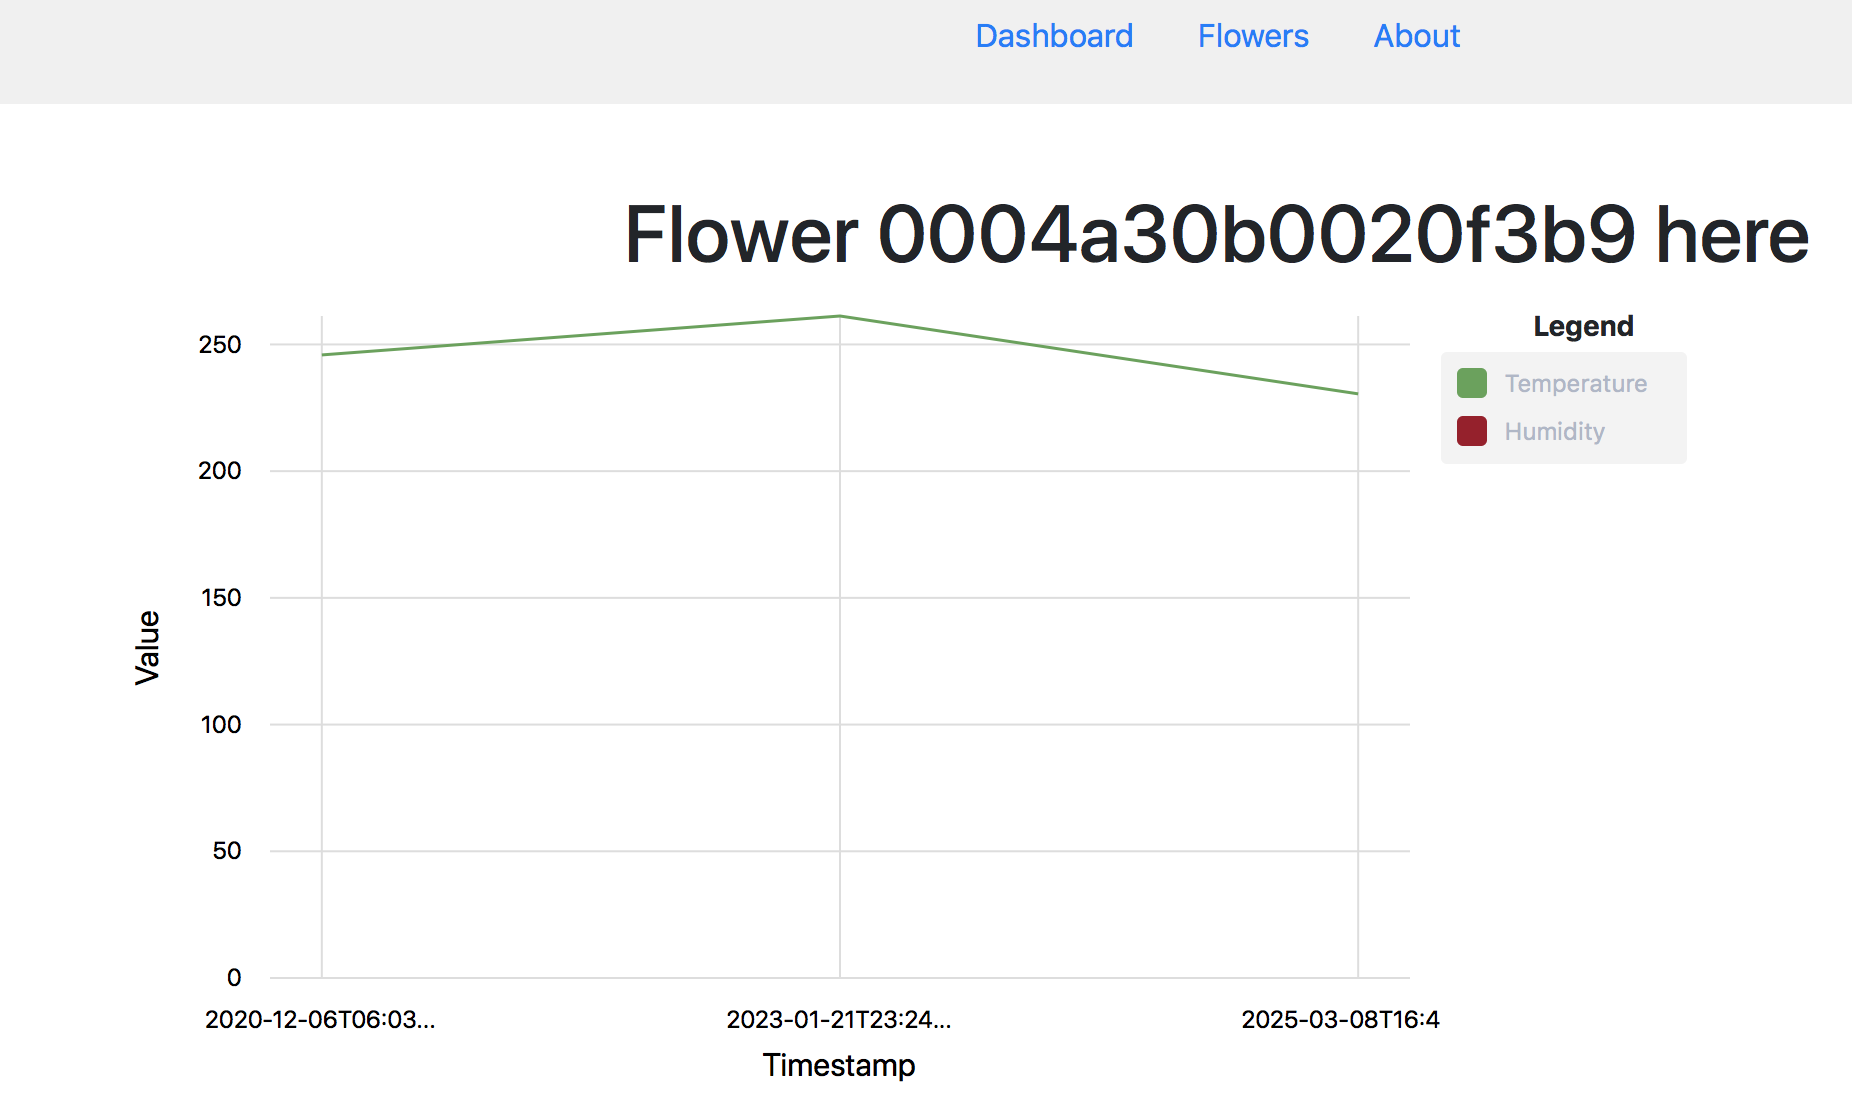
\includegraphics[width=\linewidth]{flowers}
	\caption{Sample detail page for a SunFlower}
	\label{figure:flower}
\end{figure}

% Quick intro into the tech behind the dashboard
The dashboard is built using web-technologies of which are \href{www.angular.io}{AngularJS} for the architecture and \href{https://swimlane.github.io/ngx-charts/}{Ngx-Charts} for the visualisations. The dashboard supports single-page apps and by default offline mode; highlighting the strong technologies used for the project.

% Currently supports one way communication i.e Flower => Server => Dashboard but support for bilateral comms could be added in the future
Currently the dashboard only receives data from the central server as data currently flows from the sun-flowers to the server and then to the dashboard. In the future, bilateral communication could be added; In figure \ref{figure:flower}, the sample page for a sun-flower is shown there, a sample feature that could be added would be a button to shutdown the flower where this command propagates from the dashboard to the central server and then to the sun-flower.



\subsection{Central Server}
%TODO - Quick intro in the tech behind the server (highly scalable and asynchronous in nature)
%TODO - Functionality of the server: Node serial port communication and parsing, saving to disk, processing the data for analytics
%TODO - REST API exposed which can be used by mobile apps, web-apps etc
%TODO: Include an image of the entire pipeline

\section{Mechanical Design}
\input{mech.tex}

\section{Conclusion and Future Work}


% Can use something like this to put references on a page
% by themselves when using endfloat and the captionsoff option.
\ifCLASSOPTIONcaptionsoff
  \newpage
\fi



% trigger a \newpage just before the given reference
% number - used to balance the columns on the last page
% adjust value as needed - may need to be readjusted if
% the document is modified later
%\IEEEtriggeratref{8}
% The "triggered" command can be changed if desired:
%\IEEEtriggercmd{\enlargethispage{-5in}}

% references section

% can use a bibliography generated by BibTeX as a .bbl file
% BibTeX documentation can be easily obtained at:
% http://mirror.ctan.org/biblio/bibtex/contrib/doc/
% The IEEEtran BibTeX style support page is at:
% http://www.michaelshell.org/tex/ieeetran/bibtex/
%\bibliographystyle{IEEEtran}
% argument is your BibTeX string definitions and bibliography database(s)
%\bibliography{IEEEabrv,../bib/paper}
%
% <OR> manually copy in the resultant .bbl file
% set second argument of \begin to the number of references
% (used to reserve space for the reference number labels box)
\printbibliography



% that's all folks
\end{document}


